
\section{Streaming Readout Upgrade for the sPHENIX trackers}
 
\subsection{Introduction}

As proposed in Chapter~\ref{chap:beam_use_proposal}, the sPHENIX data taking will start with \auau collisions in 2023, followed \pp and \pau collisions in 2024. Many sPHENIX observables, such as photon and jets, leave clear signature in the calorimeter system that can be used to produce a level-1 trigger. However, further physics opportunities present in the non-triggerable data, such as the low \pt open heavy flavor hadrons that decay hadronically that leaves  relatively small signals in the
calorimeters when compared with the underlying event. Therefore, they
cannot be efficiently collected via calorimeter triggers, which have a
hadron energy threshold of 10~GeV. In the 15~kHz sPHENIX trigger
bandwidth, one would only reasonably request around few kHz of the
minimum bias \pp trigger bandwidth for this new program. Assuming a
vertex range selection purity of 50\%, a 1~kHz minimum bias trigger
leads to recording $2\times10^{-4}$ of the delivered luminosity. This
translates to rather limited statistics for these rare low-$p_T$ HF
signals as quantified in Table~\ref{tab:HFppreach}.

{\textcolor{red}{REMOVE TOO MANY SPECIFIC NUMBERS FROM HERE...}}

% In the first three years of sPHENIX operation, the collaboration
% envisions a run plan sampling 2 trillion \pp collisions (50~\pb) with
% electron and jet triggers, as well as recording 140 billion M.B. \AuAu
% collisions. Comparison of HF observables in heavy-ion collisions to
% those in \pp reveals how the HF probes interact with QGP.  However,
% due to the rareness of the HF signals in the \pp collisions, the
% currently envisioned sPHENIX detector equipped with a traditional
% triggered DAQ cannot efficiently sample HF production below a $p_T$ of
% 10~GeV$/c$.
 
A study~[{\textcolor{red}{SRO tech note}}] found that the sPHENIX tracking detectors can
be upgraded to record a large amount of \pp collisions via a streaming
readout upgrade in the data acquisition (DAQ) firmware and software.
{\textcolor{red}{(Embed something we want PAC to write in report)}} 



 
% The currently envisioned sPHENIX experiment is designed to take large
% statistics of calorimeter triggered events in the \pp collisions. 
% For observables that utilize the
% calorimeters for analysis, a trigger can usually be designed, such as
% leptonic decays at higher $p_T$, jets, photon, and their correlation
% observables.  
% However, low-$p_T$ ($<10$~GeV$/c$) HF hadrons usually
% decay hadronically and leave relatively small signals in the
% calorimeters when compared with the underlying event. 




\begin{sidewaystable}[thbp]
    \centering
    \begin{tabular}{|c|c|c|c|c|c|} \hline
         & 
         & Year-2, 0-crossing  
         & Year-2, 2mrad-crossing  
         & Year-2, 
         & Year-2 and 4  \\ 
         & 
         & in current setup  
         & in current setup  
         & w/ str. tracker
         & w/ str. tracker \\            
         & 
         & Per-5kHz M.B. trigger 
         & per-5kHz M.B. trigger 
         & 
         &  \\ \hline \hline

        M.B.  & Data  
        & Each 1k Hz M.B.  
        & Each 5k Hz M.B.  
        & 10\% M.B. events 
        & 10\% M.B. events \\ 
        p+p & Mode 
        & trigger w/ $2\times10^{-4}$ 
        & trigger w/ $2\times10^{-4}$  
        & str. recorded
        & str. recorded \\ 
         &  
        & of M.B. coll. triggered 
        & of M.B. coll. triggered 
        & 
        & \\ \hline
       
         & Stats 
        & 0.4 Billion M.B. evts 
        & 13 Billion M.B. evts  
        & 200 Billion M.B. evts
        & 800 Billion M.B. evts \\ 
         &  
        & 0.01~\pb recorded 
        & 0.15~\pb recorded 
        & 5.0~\pb recorded
        & 20.0~\pb recorded \\ \hline  
        
        Physics  
        & B $\rightarrow$ D$^{0}$ $\rightarrow$ $\pi$K 
        & 250 evts  
        & 3800 evts
        & 120k evts 
        & 500k evts \\ 
        Reach &  R$_{AA}$ ref.
        &   
        &  
        & 
        &  \\ \hline          

        & 
        D$^{0} \rightarrow$ $\pi$K pair
        & 250 evts  
        & 3800 evts
        & 120k evts 
        & 500k evts \\ 
         &  Diffusion of c+$\overline{c}$
        &   
        &  
        & 
        &  \\ \hline 
 
         & 
        $\Lambda_{c} \rightarrow$ $\pi$K$p$ 
        & 500 evts  
        & 8k evts
        & 250k evts 
        & 1M evts \\ 
         &  Charm hadronization
        &   
        &  
        & 
        &  \\ \hline 
        
        &
        Prompt D$^{0} \rightarrow$ $\pi$K  
        & 75k evts  
        & 1.1M evts
        & 40M evts 
        & 150M evts \\ 
         & Tri-Gluon Corr. via SSA 
        &   
        &  
        & 
        &  \\ \hline 
        
    \end{tabular}
    \caption{Statistical reach for Heavy Flavor \pp measurements by channel in different data taking periods and modes, including streaming readout of the tracker.}
    \label{tab:HFppreach}
\end{sidewaystable}
 




 
 
\subsection{Hybrid Trigger-Streaming Readout in Run24}
 


\begin{figure}[htbp]
\begin{center}
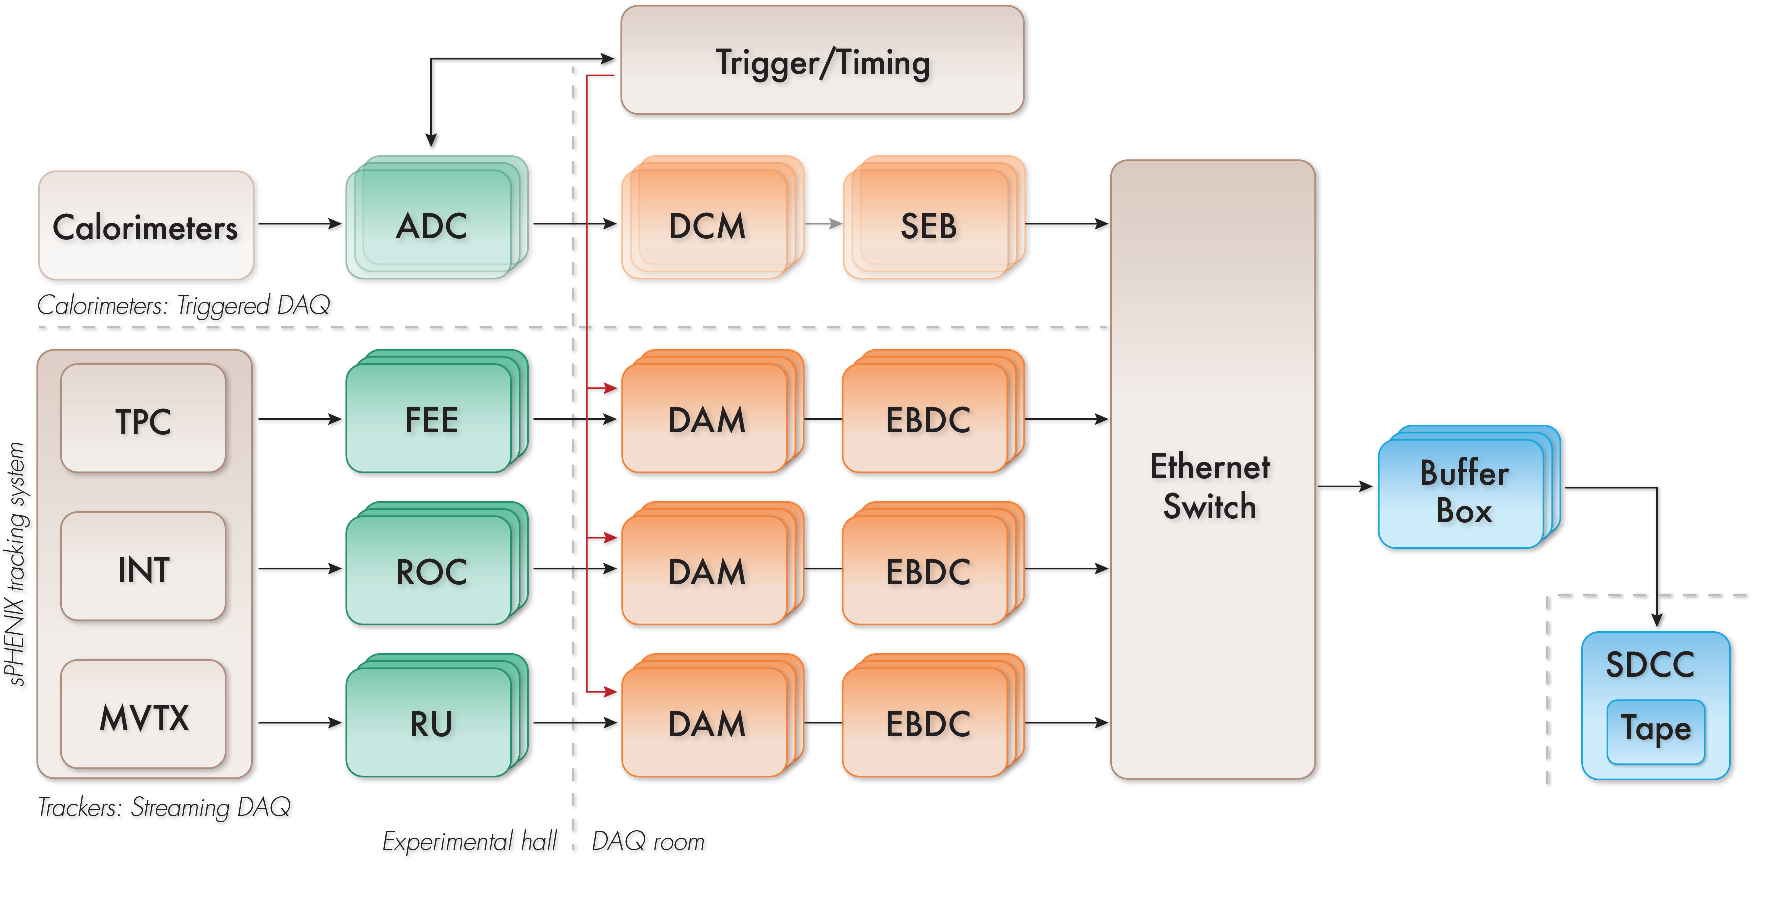
\includegraphics[width=.7\linewidth]{figs/DAQ structure_rev3.pdf}
\caption{The hybrid DAQ structure of the sPHENIX tracking detector, in which  all three tracking detectors are in streaming readout mode. The output of the tracker data stream are throttled to be in synchronize with calorimeter trigger. Additional tracker data can also be streaming to record more minimum bias collisions in addition to the calorimeteric triggered events.}
\label{fig:TPC-DAQ-structure}
\end{center}
\end{figure}
\begin{figure}[htbp]
\begin{center}
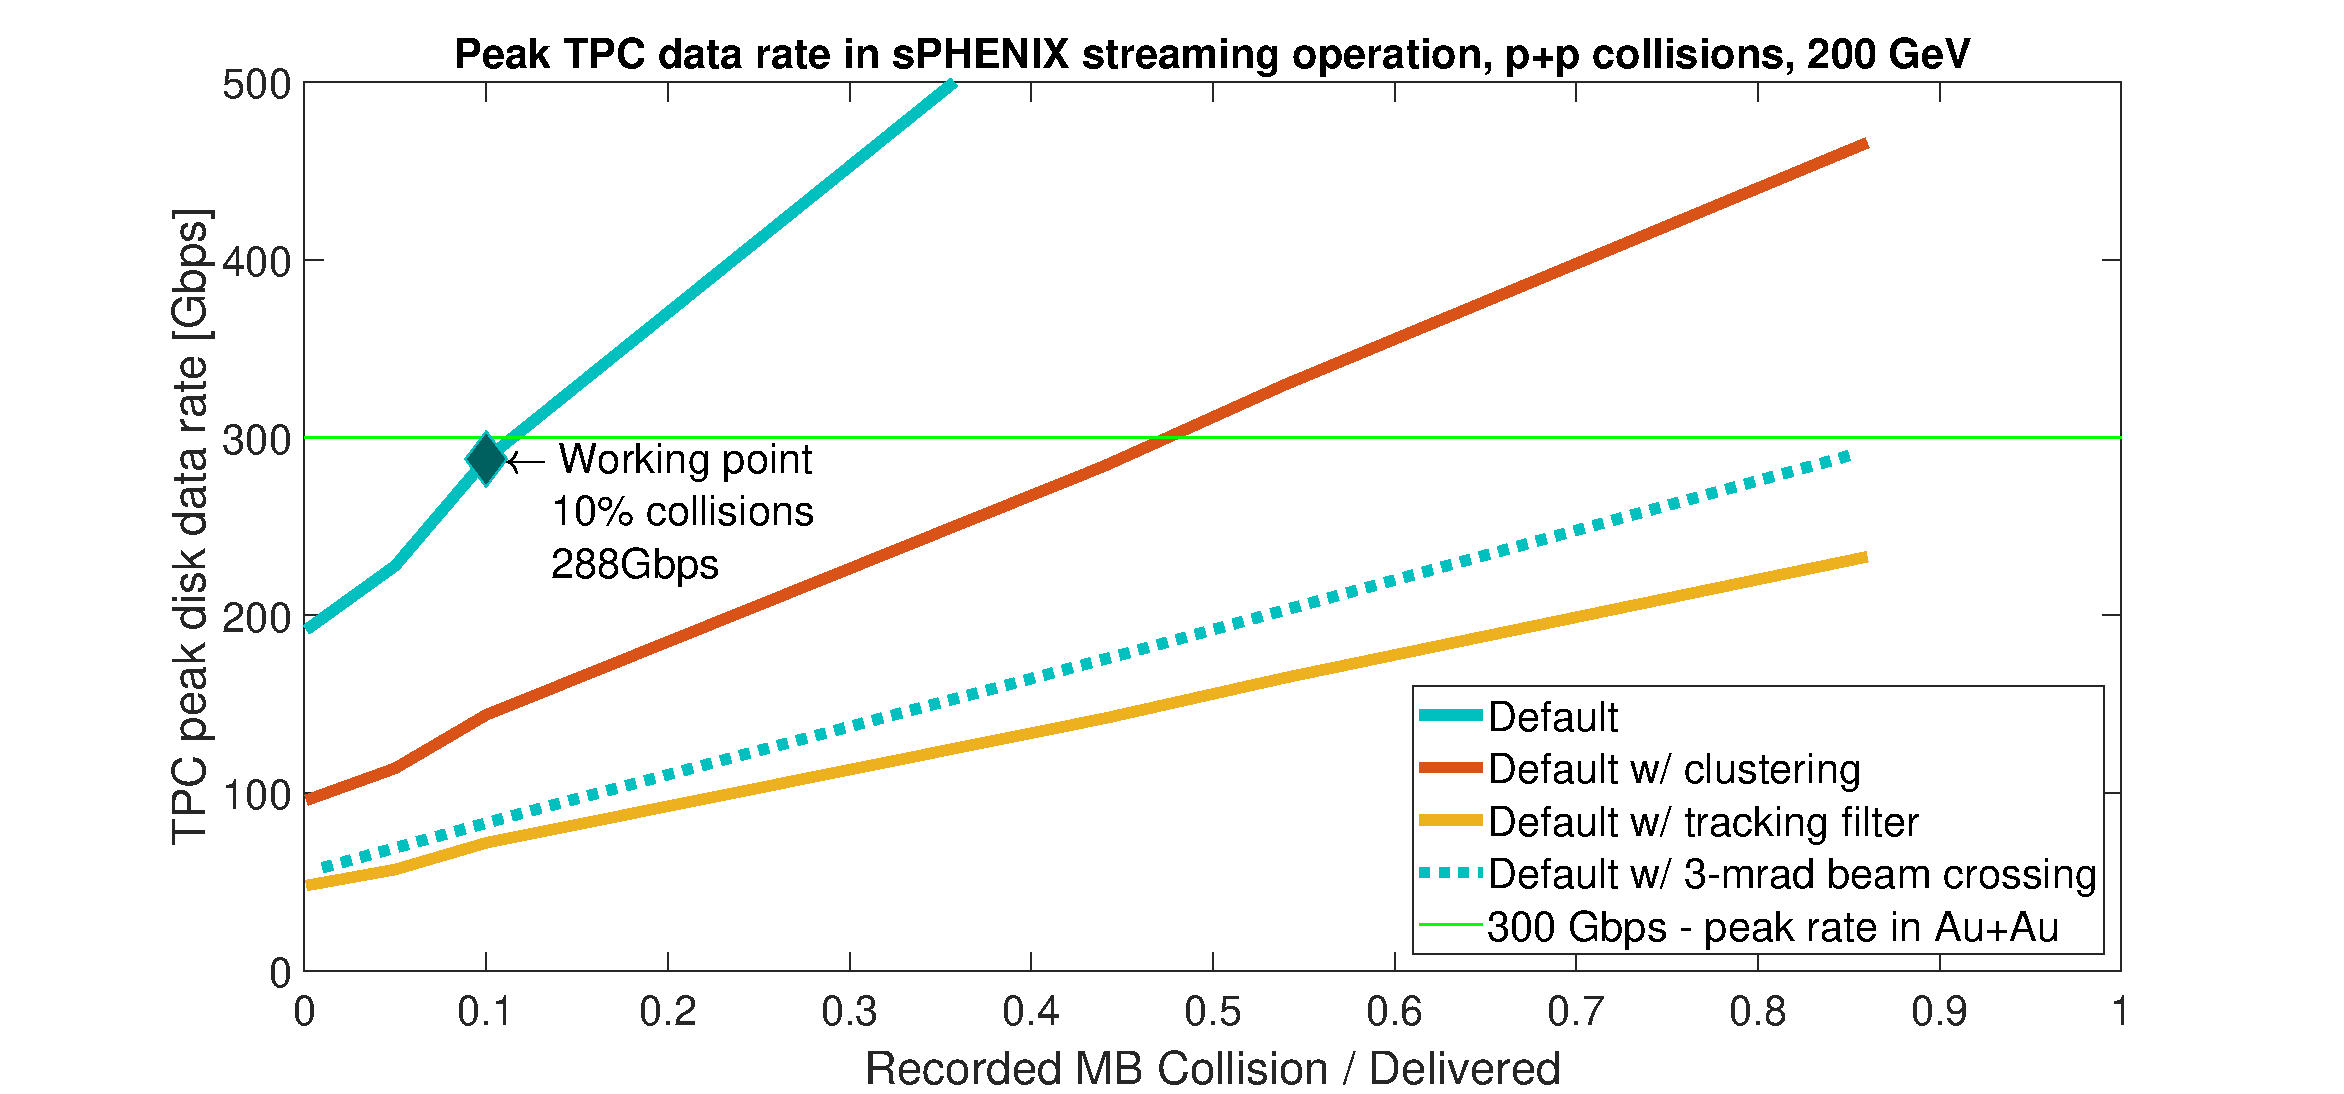
\includegraphics[width=.7\linewidth]{figs/TPCRateLayeredPP_Summary_13MHz_TriggerWindowRateCoverageCompile.pdf}
% \caption[hoice of operation point between the peak TPC data logging rate and
%   the fraction of M.B. p+p collision recorded.]{\label{fig:TPCRateWindow}
%   Choice of operation point between the peak TPC data logging rate and
%   the fraction of M.B. p+p collision recorded. The green horizontal
%   line denotes the peak data logging rate for Au+Au collisions. At
%   similar logging rate, a minimum of 10\% of \pp M.B. collisions can
%   be streamed to the raw data file as denoted by the solid cyan
%   curve. Other curves denote various online data reduction and beam
%   optimization strategies which would allow recording much higher
%   statistics at a fixed logging rate as further discussed in the last
%   Chapter X.}
\caption{Choice of operation point between the peak TPC data logging rate and the fraction of M.B. p+p collision recorded. The green horizontal line denotes the peak data logging rate for Au+Au collisions. At similar logging rate, a minimum of 10\% of \pp M.B. collisions can be streamed to the raw data file as denoted by the solid cyan curve. In the case that a cross angle is introduced (dashed cyan curve) the overall data rate can be significantly reduced. Various online data reduction strategy could further reduce the data rate too as presented by the red and orange curves.}
\label{fig:TPC-DAQ-rate}
\end{center}
\end{figure}
 
The upgraded DAQ is illustrated in Figure~\ref{fig:TPC-DAQ-structure} and
summarized in Table~\ref{tab:HFppreach}.  The FEE and DAQ hardware of
each of the three tracking detectors supports a streaming readout mode
and provides the capability needed for this upgrade. The main work
will focus on DAQ firmware and software development that enabling the
streaming capability.  This upgrade would enable the collection of
sufficient minimum bias in \pp events.  That is, 10\% delivered
luminosity (see next Chapter) or 200~billion events in the acceptance
of the vertex tracker, which is a factor of 500 improvement. This
dataset enables a comprehensive low-$p_T$ hadron program as discussed
here.  The analysis of these HF hadronic channels does not require
calorimeter information. Instead, they can be identified with the precision
tracking detectors of sPHENIX (at $p_T=5$~GeV$/c$, $\sigma(p)/p=1\%$,
$\sigma(DCA)<10$~$\mu$m ) via a combination of decay topology and
invariant mass, as demonstrated for even the busiest events of Au+Au
collisions through detailed simulation studies in~\cite{sPH-HF-2017-002}.

As summarized in Table~\ref{tab:HFppreach}, an upgraded DAQ for
sPHENIX trackers will enable the recording of 500 times greater
statistics of M.B. \pp collisions, which in turn will enable proper HF
measurements in this key kinematic region.

\subsection{Full streaming Readout in Run26}

[Readout everything in tracker]

\subsection{Data Preservation and Data Mining}

This upgrade will accumulate a large amount (10-100\% of delivered luminosity) 
of minimum
bias polarized \pp collision without a trigger bias and with the full
sPHENIX tracking capability. After RHIC completes its scientific
mission at the end of the sPHENIX program, this would be a unique
dataset allowing future data mining for novel quantum effects such as
the quantum coherence in particle productions. These \pp data may be
critical in understanding the future $e+p/A$ collision data at an
EIC~\cite{Accardi2012}.
